% !TEX root = ../sbgn_ER-level1.tex
%\color{red}
\section{Semantic description of \ERs}

% Add small images of the glyphs

\subsection{Entities and states}

An \glyph{entity} (\sect{entity}) represents a set of individual instances of some kind (molecules, agents etc). The difference from \SBGNPDLone \glyph{entity pool node} is that \glyph{entity} instances are independent, while \glyph{entity pool node} form one inseparable object acting as a whole. A set of \glyph{state variables} (\sect{stateVariable}) and their \glyph{values} (\sect{variableValue}) describe a part of the \glyph{entity} instances state space. The  \glyph{entity}, or  interaction \glyph{outcome} (\sect{outcome}) acquire the true state if the set of entity instances compatible with the \glyph{entity} state, or  actualisation of interaction is non-empty. 

 
\subsection{Statements}

An \glyph{interaction} (\sect{interaction}) linking the \glyph{interactors} $A$ and $B$ means: ``any instance of $A$ can interact with instances of $B$''. An \glyph{outcome} on an \glyph{interaction} represents the cases when the statement is true, that is subset of all instances of $A$ and $B$ between which the interaction effectively exists. If the interaction is a physical interaction between molecules, the \glyph{outcome} represents all possible complexes where interactors are really bound to each other, and in that case interaction is always considered as reversible. It is used as follow: ``when (or if) $A$ interacts with $B$ then \ldots''.\\[\baselineskip]

\noindent
An \glyph{assignment} (\sect{assignment}) linking a \glyph{variable value} $v$ to a \glyph{state variable} $V$ of an \glyph{entity} $E$ means: ``$v$ is assigned to $V$ of $E$'' or ``$V$ of $E$ takes the value $v$''. An \glyph{outcome} on an \glyph{assignment} represents the cases when the statement is true, that is all instances of $E$ (free or as a complex subunint) on which the variable effectively displays the value. It is used as follows: ``when (or if) $V$ of $E$ takes the value $v$ then \ldots'' or more succintly ``when (or if) $E\{V => v\}$ then \ldots''.\\[\baselineskip]

%\noindent
%A \glyph{phenotype} (\sect{phenotype}) $P$ means: ``$P$ exists''.\\[\baselineskip]

\subsection{Influences}

A \glyph{modulation} (\sect{modulation}) linking an \glyph{entity node} (\sect{ENs}) $E$  and a relationship $R$ means: ``If $E$ exists then $R$ is either reinforced or weakened''. 
%An \glyph{outcome} on a \glyph{modulation} represents the cases when the modulation effectively takes place. It is used as follow: ``when (or if) $I$ modulates $R$ then \ldots''.
\\[\baselineskip]

\noindent
A \glyph{stimulation} (\sect{stimulation}) linking an \glyph{entity node} (\sect{ENs}) $E$ and a relationship $R$ means: ``If $E$ exists then $R$ is reinforced'' or ``If $E$ exists then the probability of $R$ is increased''. 
%An \glyph{outcome} on a \glyph{stimulation} represents the cases when the stimulation effectively takes place. It is used as follow: ``when (or if) $I$ stimulates $R$ then \ldots''.
\\[\baselineskip]

\noindent
An \glyph{absolute stimulation} (\sect{absoluteStimulation}) linking an \glyph{entity node} (\sect{ENs}) $E$ and a relationship $R$ means: ``If $E$ exists then $R$ always takes place with necessity''. 
\\[\baselineskip]

\noindent
A \glyph{necessary stimulation} (\sect{necessaryStimulation}) linking an \glyph{entity node} (\sect{ENs}) $E$ and a relationship $R$ means: ``$R$ only takes place if $E$ exists. 
%An \glyph{outcome} on a \glyph{necessary stimulation} represents the cases when the stimulation effectively takes place. It is used as follow: ``when (or if) $I$ allows $R$ then \ldots''.
\\[\baselineskip]

\noindent
An \glyph{inhibition} (\sect{inhibition}) linking an \glyph{entity node} (\sect{ENs}) $E$ and a relationship $R$ means: ``If $E$ exists then $R$ is weakened'' or ``If $E$ exists then the probability of $R$ is lowered''. 
%An \glyph{outcome} on an \glyph{inhibition} represents the cases when the inhibition effectively takes place. It is used as follow: ``when (or if) $I$ inhibits $R$ then \ldots''.
\\[\baselineskip]

\noindent
An \glyph{absolute inhibition} (\sect{absoluteInhibition}) linking an \glyph{entity node} (\sect{ENs}) $E$ and a relationship $R$ means: ``If $E$ exists then $R$ never takes place''. 
%An \glyph{outcome} on an \glyph{absolute inhibition} represents the cases when the absolute inhibition effectively takes place. It is used as follow: ``when (or if) $I$ blocks $R$ then \ldots''.
\\[\baselineskip]

\subsection{Logical Operators}

An \glyph{and} (\sect{and}) linking several \glyph{logic arcs} originating from \glyph{entity nodes} (\sect{ENs}) $E_i$ and an influence $F$ means: ``if for each $i$, $E_i$ exists, then $F$''.\\[\baselineskip]

\noindent
An \glyph{or} (\sect{or}) linking several \glyph{logic arcs} originating from \glyph{entity nodes} (\sect{ENs}) $E_i$ and an influence $F$ means: ``if for any $i$, $E_i$ exists, then $F$''.\\[\baselineskip]

\noindent
A \glyph{not} (\sect{not}) linking a \glyph{logic arc} originating from an \glyph{entity node} (\sect{ENs}) $E$ and an influence $F$ means: `` $F$ takes place only if $E$ does not exist''.\\[\baselineskip]

%\noindent
%A \glyph{delay} (\sect{delay}) linking a \glyph{logic arc} originating from an \glyph{entity node} $E$ and an influence $F$ means: ``If $E$ exists then $F$ takes place, but not immediately''.\\[\baselineskip]

\subsection{Cis and trans relationships}\label{sec:cis-trans-semantics}

The use of cis and trans units of information on a combination of relationships brings power and versatility to \ERs. However, the resulting semantics may be difficult to grasp. Here are the basic rules that permit to understand the graphs.

\begin{itemize}
 \item The unit of information ``cis'' or ``trans'' carried by an \glyph{interaction} refers to the \glyph{interactors} targeted by the \glyph{interaction}. 
 \item The unit of information ``cis'' or ``trans'' carried by an \glyph{influence} targeting a state variable \glyph{assignment} refers to the origin of the \glyph{influence} and to the \glyph{entity} carrying the target of the \glyph{assignment}. 
\item The unit of information ``cis'' or ``trans'' carried by an \glyph{influence} targeting another \glyph{influence} refers to the origin of the carrying \glyph{influence} and to the origin of the targeted \glyph{influence}.
 \item The unit of information ``cis'' or ``trans'' carried by an \glyph{influence} targeting an \glyph{interaction} refers to the origin of the \glyph{influence} and all the relevant \glyph{interactors} targeted by the \glyph{interaction} (see \sect{SyntacticRules}).
\end{itemize}

\subsection{Use of nested entities}\label{sec:semanticsDomain}

\noindent
The relationship between an \glyph{entity} and the \glyph{entities} it contains is a partonomy (meronymy). Any instance of the contained \glyph{entity} is part of an instance of the containing \glyph{entity}.

\noindent
No functional relationship are implied between \glyph{entities} that are part of the same \glyph{entity}. Such relationships if any must be explicit. In particular, there is no implied disjunction.

\noindent
\glyph{Entity nesting} is transitive. If $E1$ contains $E2$ and $E2$ contains $E3$, then any instance of $E3$ is part of an instance of $E2$ and any instance of $E2$ is part of an instance of $E1$, therefore any instance of $E3$ is part of an instance of $E1$.

\noindent
The assignment of a certain value to the variable \glyph{location} of the containing \glyph{entity} effectively assigns this value to the variable \glyph{location} of all contained \glyph{entities}. For instance, a protein that translocates from the cytosol to the nucleus causes the translocation of all its domains.

\noindent
The assignment of a certain value to the variable \glyph{location} of a contained \glyph{entity} does not assign this value to the variable \glyph{location} of the containing \glyph{entity}. For instance a protein domain can translocate from the cytosol into the plasma membrane, but the whole protein still belong to the cytosol.

\begin{figure}[H]
  \centering
  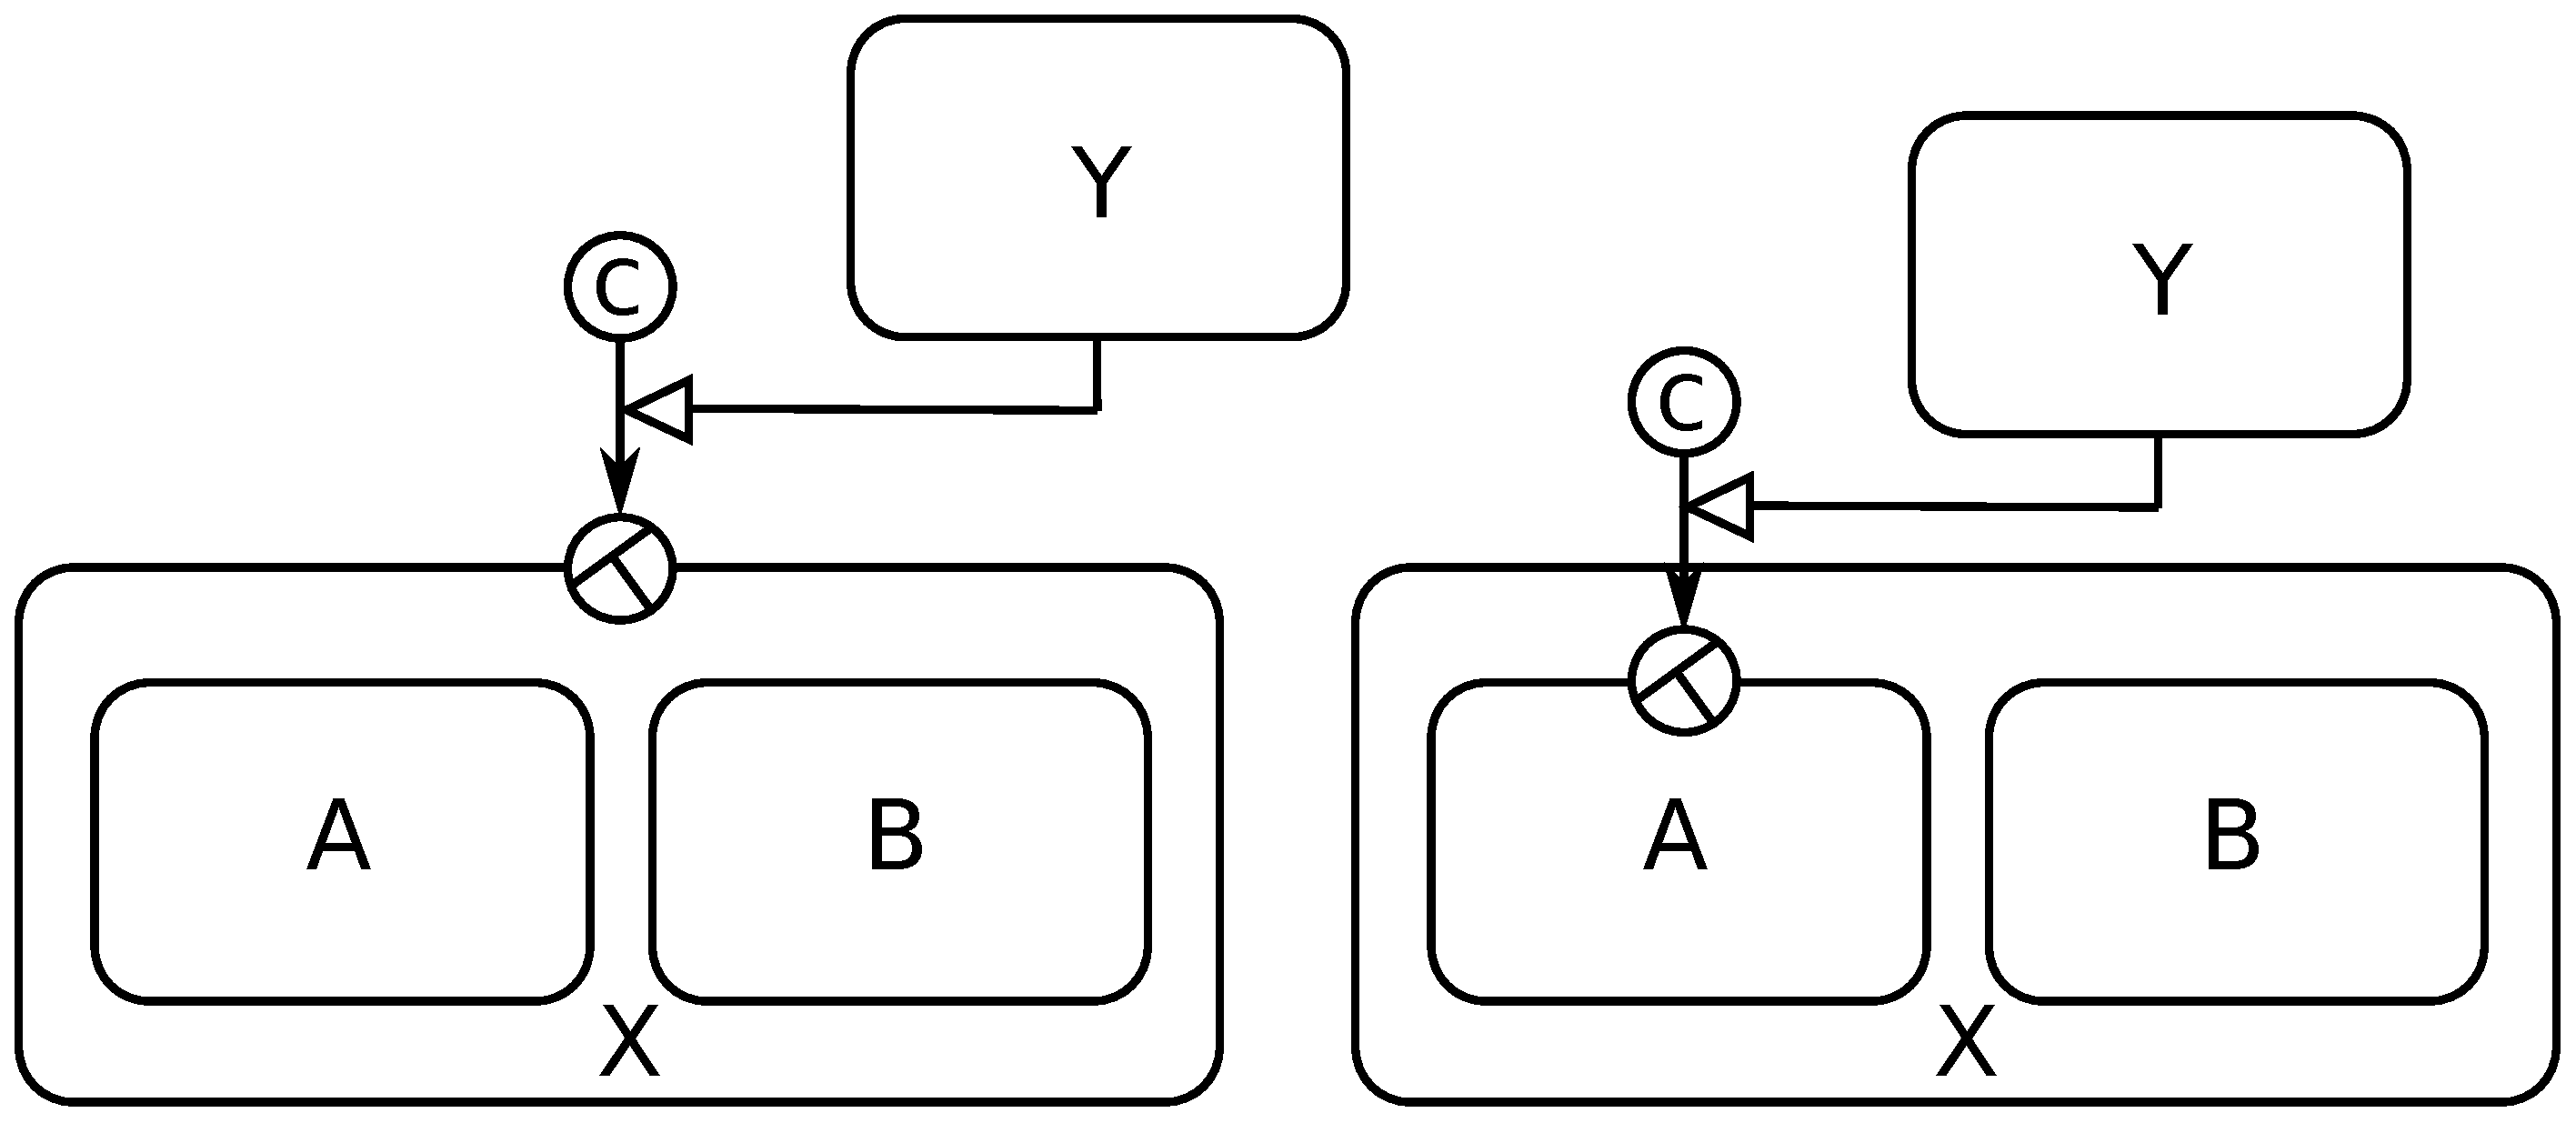
\includegraphics[scale = 0.3]{images/nesting-location}
  \caption{On the left, the entity Y causes the whole entity X to translocate to the location c, including its A and B components. On the right, only the entity A is translocated, without effect on B and X.}
  \label{fig:nesting-location}
\end{figure}


\noindent
The assignment of a certain value to the variable \glyph{existence} of the containing \glyph{entity} effectively assigns this value to the variable \glyph{existence} of all contained \glyph{entities}. For instance, the degradation of a protein implies the degradation of all its domains.

\noindent
The assignment of a certain value to the variable \glyph{existence} of a contained \glyph{entity} does not assign this value to the variable \glyph{existence} of the containing \glyph{entity}. For instance the degradation of a protein domain does not imply the degradation of the entire protein.

\begin{figure}[H]
  \centering
  \includegraphics[scale = 0.3]{images/nesting-existence}
  \caption{On the left, the entity Y causes the disappearance of the whole entity X, including its A and B components. On the right, only the entity A disappear, without effect on B and X as a whole.}
  \label{fig:nesting-existence}
\end{figure}

Outcome of an interaction that involves contained entities is defined along the same line as in \sect{outcome}: the outcome represents set of all possible instances of topmost containing entity has domains represented by contained entity involved in interaction.

\subsection{(In)Validation of ER maps}

Based on the definitions above, it should be possible to use the toolkit of formal logic to analyse \ERs{}. In particular, one can envision to build truth tables describing the consequences of the existences of the various entities. Those tables should point to inconsistencies leading to contradictory predicates.

% Give an example of a wrong ER map.

%\normalcolor

